\section{Experiment}
We will experiment with our system upon the validation dataset and compare it with the baseline.
\subsection{Validation Period}
To verify that our system is stable, we validate our system on two different validation periods. 
\begin{table}[htb]
    \centering
    \begin{tabular}{|c|c|c|c|c|}
    \hline
    \multirow{2}{*}{Period} &
    \multirow{2}{*}{Start} &
    \multirow{2}{*}{End} &
    \multicolumn{2}{c|}{S\&P 500} \\ 
    \cline{4-5} &{} &{} & CAGR & MDD \\ \hline
    Period 1 & 2017/3/1 & 2019/2/28 & 7.81\% & 19.78\% \\ \hline
    Period 2 & 2019/3/1 & 2021/3/15 & 18.56\% & 33.9\% \\    
    \hline
    \end{tabular}
    \caption{Validation Period}
    \label{tab:validation_period}
\end{table}
\begin{figure}
    \centering
    \includegraphics{}
    \caption{Caption}
    \label{fig:my_label}
\end{figure}



\subsection{Baseline}
A Constant rebalanced portfolio (CRP) is an investment strategy that keeps a constant ratio between all investments over time. We use this to represent the portfolio provided by advisors to meet investors' risk preferences. We will use the average ratio of our portfolio to build a CRP portfolio and use it as a baseline for performance comparison in MDD and CAGR.
\subsection{Threshold}
We will test three different thresholds to represent risk preferences.  
\begin{table}[htb]
    \centering
    \begin{tabular}{|c|c|}
    \hline \hline
    Threshold $\theta$ & Risk Preference \\ \hline
    $\infty$  (no plenty) & High \\ \hline
    0.006 & Medium      \\ \hline
    0.002 & Low      \\ \hline    
    \hline
    \end{tabular}
    \caption{Threshold and Risk Preferences}
    \label{tab:threshold}
\end{table}
\subsection{Result}
We experiment our models with different thresholds and compare with constant rebalanced portfolio (CRP). 
CRP is a portfolio policy that maintain the weights thoughtout the trading period. 
Our system successfully delivers portfolios with different MDD to meet various investors' preferences, and output performed CRP in MDD and CAGR in most situations.

\begin{figure}[htb]
\centering
  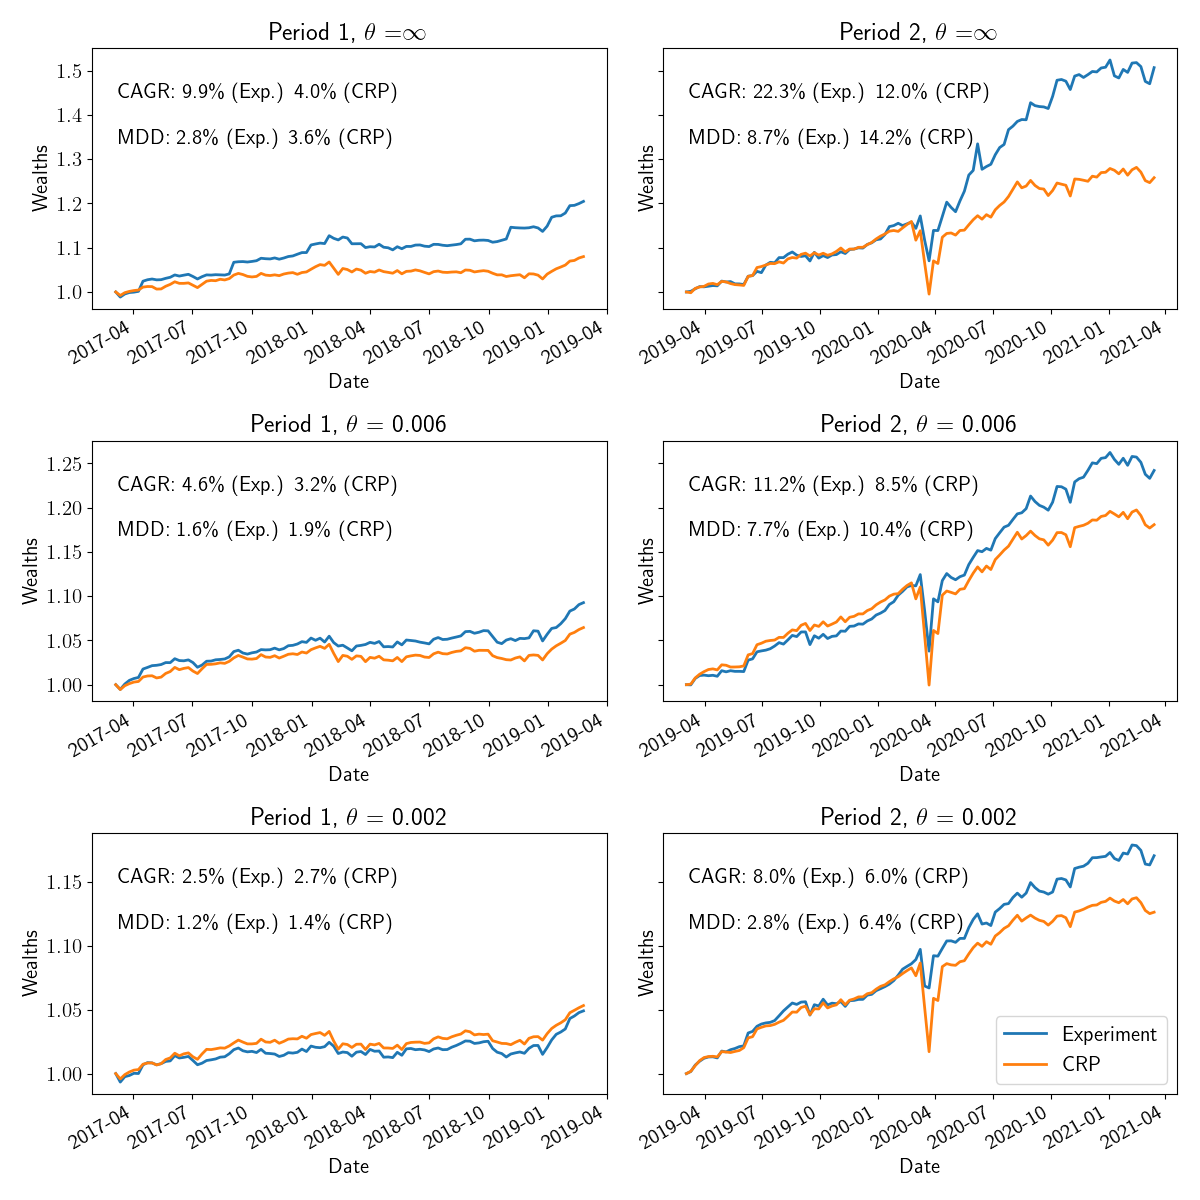
\includegraphics[width=16cm]{images/crp_compare.png}
  \caption [Comparison of experiments result with CRP]{Comparison of experiments result with CRP}
  \label{fig:crp_compare}
\end{figure}